
%!TEX encoding = UTF-8 Unicode
%----------------------------------------------------------------------------------------
%	PACKAGES AND OTHER DOCUMENT CONFIGURATIONS
%----------------------------------------------------------------------------------------

\documentclass[11pt, a4paper, oneside]{Thesis} % Paper size, default font size and one-sided paper
% Para adicionar a língua (PT)
\usepackage[portuges]{babel}
% suporte para utf8
\usepackage[utf8]{inputenc}
\usepackage{aeguill}
\usepackage{multirow}
\usepackage{color}


\usepackage{listings}				%package to show code

\usepackage{comment}
\usepackage{mathtools}			%mathematic tools

\graphicspath{{./Pictures/}} % Specifies the directory where pictures are stored
\usepackage[square, numbers, comma, sort&compress]{natbib} 
\hypersetup{urlcolor=blue, colorlinks=true} % Colors hyperlinks in blue - change to black if annoying
\title{\ttitle} % Defines the thesis title - don't touch this


\renewcommand{\labelitemi}{$\bullet$}   %Tipo de bullet points utilizados nas enumerações
\begin{document}

\frontmatter % Use roman page numbering style (i, ii, iii, iv...) for the pre-content pages

\setstretch{1.2} % Line spacing of 1.3

% Define the page headers using the FancyHdr package and set up for one-sided printing
\fancyhead{} % Clears all page headers and footers
\rhead{\thepage} % Sets the right side header to show the page number
\lhead{} % Clears the left side page header

\pagestyle{fancy} % Finally, use the "fancy" page style to implement the FancyHdr headers

\newcommand{\HRule}{\rule{\linewidth}{0.5mm}} % New command to make the lines in the title page

\definecolor{dkgreen}{rgb}{0,0.6,0}
\definecolor{gray}{rgb}{0.5,0.5,0.5}
\definecolor{mauve}{rgb}{0.58,0,0.82}
%----------------------------------------------------------------------------------------
%	TITLE PAGE
%----------------------------------------------------------------------------------------

\begin{titlepage}
\begin{center}

\textsc{\LARGE \univname}\\[2cm] % University name
\textsc{\Large Computação em Nuvem }\\[0.5cm] % Major heading such as course name
\textsc{\large Grupo 6 }\\[1cm] % Minor heading such as course title


\HRule \\[0.4cm] % Horizontal line
{\huge \bfseries CloudWeather }\\[0.4cm] % Thesis title
\HRule \\[1.5cm] % Horizontal line
 
 \Large 
 65963 - David \textsc{Dias}\\[0.5cm] 
 68206 - Artur \textsc{Balanuta}\\[0.5cm] 
68210 - Dário \textsc{Nascimento}\\[8cm] 


\Large 17 de Novembro de 2012\\[3cm] 

\vfill
\end{center}

\end{titlepage}
%----------------------------------------------------------------------------------------
%	LIST OF CONTENTS/FIGURES/TABLES PAGES
%----------------------------------------------------------------------------------------

\pagestyle{fancy} % The page style headers have been "empty" all this time, now use the "fancy" headers as defined before to bring them back

\lhead{\emph{Índice}} % Set the left side page header to "Contents"
\tableofcontents % Write out the Table of Contents

\clearpage % Start a new page



%----------------------------------------------------------------------------------------
%	THESIS CONTENT - CHAPTERS
%----------------------------------------------------------------------------------------

\mainmatter % Begin numeric (1,2,3...) page numbering

\pagestyle{fancy} % Return the page headers back to the "fancy" style

% Include the chapters of the thesis as separate files from the Chapters folder
% Uncomment the lines as you write the chapters

%!TEX encoding = UTF-8 Unicode
% Chapter 1

\chapter{Introdução} % Main chapter title

\label{Chapter1} % For referencing the chapter elsewhere, use \ref{Chapter1} 

\lhead{Chapter 1. \emph{Introdução}} % This is for the header on each page - perhaps a shortened title

%----------------------------------------------------------------------------------------

dfsfndfdsfldsufahsiudhfasid

No âmbito da disciplina de Computação em Nuvem foi desenvolvido um projecto designado de “Cloud Weather” com objetivo de analisar dados produzidos por sensores de humidade, temperatura e precipitação, calculando os mínimos, máximos e a médias de temperatura e humidade, tal como a quantidade total de precipitação de vários pontos geográficos, com especial atenção sobre cidades.\\
Com o aumento da informação produzida pelos sensores e utilizadores nos sistemas de informação, a recolha e processamento de dados assume uma enorme preponderância nas tecnologias de informação atuais. \\
Nos últimos anos, devido às constrições económicas houve a necessidade de aumentar a eficiência e flexibilidade dos sistemas informáticos. Surgiu um novo conceito que oferece recursos como ciclos de CPU, storage e bandwith, com um formato 'pay-as-you-go' e que hoje é conhecido como Cloud Computing.\\
\\
O Cloud Weather recebe um grande número de dados enviados por várias estações meteorológicas durante um longo período de tempo. Estes dados precisam de ser processados regularmente de forma a que a informação sobre o estado meteorológico esteja o mais atual possível. Para processar os dados que são produzidos em larga escala foi desenhado um algoritmo MapReduce que  processa os dados e resume os dados para permitir a sua visualização. Uma vez processados, os dados são guardados numa base de dados para serem acessíveis pelo utilizador da aplicação. Uma vez que o processamento dos dados termine, um utilizador do sistema Cloud Weather pode aceder à página Web do serviço par consultar a informação disponível. Assumindo que o serviço de meteorologia é requisitado por muitos utilizadores é necessário uma grande capacidade de resposta por parte da aplicação.No entanto, tal como acontece no caso de processamento de dados, estes pedidos encontram-se distribuídos de forma não uniforme durante o dia, o que significa que a solução de construir um data center para os servir resultaria num desperdício de recursos em algumas partes do dia.\\ 
Em resposta à oscilação do número de pedidos foi adoptada uma solução de "Load Balancer" um mecanismo que permite que a nossa capacidade de resposta seja elástica em função da quantidade de pedidos, isto é, serão instanciadas mais máquinas do provedor quando precisarmos de mais capacidade de resposta. A carga é distribuída pelas várias máquinas. Quando o número de pedidos diminui, as instâncias deixam de ser necessárias, por isso são descartadas.  \\
A vantagem da utilização de um provedor de  Cloud Computing para este  sistema  consiste no facto de não ser necessário um grande investimento na construção de um cluster para processar todos estes dados e pedidos exporádicos. Em alternativa alugamos as máquinas necessárias durante o tempo necessário para fazer o processamento pretendido. Esta solução é mais económica porque reduz a necessidade de ter poder computacional sem estar a ser utilizado enquanto não é necessário processar dados. Optámos pela solução de Cloud Computing IaaS da Amazon: Amazon Elastic Cloud Computing (EC2)\\

O sistema é constítuido pelos seguintes componentes:
   \begin{itemize}
\item Ficheiro que contém todos os dados oriundos dos sensores das estações meteorológicas 
\item Unidades EC2 que tratam do processamento dos dados usando um algoritmo de MapReduce
\item Armazenamento dos dados em Base de Dados
\item Servidores Web para consulta de base de dados
\item Load Balancing dos servidores Web
\item Auto-scalling dos servidores Web
\end{itemize}
%----------------------------------------------------------------------------------------








%!TEX encoding = UTF-8 Unicode
% Chapter Template

\chapter{Estado da arte das tecnologias de computação na nuvem} % Main chapter title
\label{Chapter2} % Change X to a consecutive number; for referencing this chapter elsewhere, use \ref{ChapterX}

\lhead{Chapter 2. \emph{Estado da arte das tecnologias de computação na nuvem}} % Change X to a consecutive number; this is for the header on each page - perhaps a shortened title

%----------------------------------------------------------------------------------------
O Cloud Computing é um paradigma que veio introduzir aos serviços de computação, armazenamento, rede, segurança, entre outros disponíveis na internet, uma forma de consumo feito à medida, sendo só usado o necessário para responder à necessidade. Este não é um conceito novo, já usufrui mos dele diariamente quando utilizamos a eletricidade, água e gás das nossas casas, estes serviços são chamados de 'utilities', uma concepção que não existia na computação até a chegada do Cloud Computing. \\
As tecnologias de computação na nuvem são bastante recentes, tendo um pouco mais de 4 anos, no entanto, visto darem a possibilidade a qualquer entidade de consumir apenas a computação, armazenamento, etc que necessitam, tiveram uma grande procura que ainda hoje se mantém, com o aparecimento de bastantes negócios que tiram a vantagem de um mundo interligado através da internet, como por exemplo o mundo das aplicações movéis.\\
Nesta seção vamos descrever alguns dos 'players' mais influentes deste mercado tal como a Google, Amazon e Microsoft e ainda um dos concorrentes mais novos, a Nodejitsu. Será apresentado também as tecnologias existentes de armazenamento na Cloud e ainda uma comparação direta sobre dois dos provedores analisados para realizar este projeto.\\
É de notar ainda que existem 3 categorias majoritárias em que podemos dividir os tipos de serviços prestados pela Cloud, temos:\\
\begin{itemize}
\item {\bf IaaS(Infrastructure as a Service)} - Caracteriza-se por disponibilizar de máquinas na Cloud em que os developers têm controle sobre as mesmas, podendo criar a sua própria instalação do sistema operativo
\item {\bf PaaS(Platform as a Service) }- Dentro desta categoria entram os servidores aplicacionais e as API disponíveis para as aplicações Web
\item {\bf SaaS(Software as a Service) }- Software alojado na internet, como por exemplo o caso do Wordpress ou a Citrix que disponibilizão um leque de aplicações via browser aos seus clientes.
\end{itemize}

A Cloud trouxe alguns novos desafios para os developers com novos modelos de programação, novas API e o MapReduce que vêm a permitir o tratamento de dados por várias máquinas em simultâneo para agregar no fim os seus resultados.


\section{Os vários 'players' no mercado da computação na nuvem}

Existem 3 maiores serviços concorrentes a liderar o mercado do Cloud Computing, estes são a Amazon AWS, Windows Azure e o Google App Engine, estes aparecem a priori como candidatos a melhor escolha para implementação da nossa aplicação na Cloud, no entanto decidimos avaliar um quarto provedor, a Nodejitsu, que permite desenvolver aplicações para a nuvem usando um servidor aplicacional chamado node.js, este é completamente open source e tem uma grande comunidade a oferecer suporte.
\\

\subsection{Amazon AWS}
A Amazon foi a pioneira a introduzir no mercado 'Public Clouds', o seu serviço consiste em disponibilizar máquinas virtuais on demand com o preço ajustado ao consumo feito. \\
Tem soluções de storage em formato de bases de dados relacionais(Relational Database Service, RDS) e bases de dados NoSQL (SimpleDB que veio a ser substituído pelo DynamoDB), estas são altamente escaláveis e tolerantes a faltas e por último disponibíliza um serviço de file storage, denominado por Simple System Storage(S3).\\
Existem ainda outros serviços disponibilizados pela Amazon como o SQS, um sistema de mensagens em fila, a Elastic Cache, um sistema de cache distribuído, a CloudFront, um serviço CDN(Content Delivery Network).\\
A Amazon dispõe ainda de um 'Free Tier' que não inclui todos os seus serviços mas que dá hipótese aos programadores de terem acesso a uma plataforma de computação distribuída sem custo.\\


\subsection{Google App Engine}

O Google App Engine(GAE) levou para a Cloud ambientes de desenvolvimento já conhecidos pelos programadores como o Java e o Python, é o único dos serviços estudados que dispões de uma versão, embora de consumo limitado, completamente gratuita.\\
O modelo do GAE divide as suas máquinas em duas categorias:\\
		
\begin{itemize}
\item {\bf App Engine Instances } - Responsáveis por instanciar as aplicações web, estas não são máquinas virtuais, mas sim ambientes de execução controlados chamados de 'sandbox'
\item {\bf App Engine Backends }- Semelhantes as Instances, mas com elevada capacidade de computação, usadas para processamento de dados em background.
\end{itemize}
	
O modelo de storage do GAE é o App Engine Datastore, este garante que a aplicação se torna escálavel, sendo que os dados são replicados em grande quantidades. No entanto o modelo de storage impede que sejam utilizados serviços de terceiros para guardar informação. O storage é feito em bases de dados NoSQL, relacionais e em file system (blob storage).\\
Tem disponivél uma API para MapReduce, Channel, que permite notificações por 'push', listas de tarefas (Task Queues) e MemCache, uma memória distribuída.	

\subsection{Windows Azure}
O Windows Azure demonstra uma das taxas de crescimento mais rápido entre as nuvens públicas, fornece um serviço de Platform as a Service (Paas) rico em funcionalidade.\\
O serviço de computação disponibilizado divide-se em 3 tipos:
	
\begin{itemize}
\item {\bf Web Role} -  Máquinas dedicadas para alojar as aplicações web e para responder aos pedidos dos clientes
\item {\bf Worker Role }- Máquinas destinadas a efectuar processamentos com maior esforço
\item {\bf VM Role }- MMáquinas virtuais, estas não são persistentes
\end{itemize}	

A juntar ao serviço de computação, temos ainda acesso a um serviço de storage que se divide em:
\begin{itemize}
\item {\bf Table Storage } -  Uma base de dados altamente escalável
\item {\bf Queue Storage  }- Uma storage de filas de mensagens
\item {\bf Blob Storage }- File System Storage
\item {\bf SQL Azure }- Bases de dados relacionais preparadas para a Cloud.
\end{itemize}	

Não está disponível uma versão gratuita limitada, mas é oferecido um período de 3 meses de experimentação.\\
Outros serviços oferecidos pelo Azure são o Business Analytics que permite efetuar analises ao desempenho da nossa aplicação, Caching e um Content Delivery Network que trata de mover a nossa informação para o local onde se deve encontrar para diminuir o delay nas respostas.


\subsection{Nodejitsu}
A Nodejitsu, ao contrário dos provedores descritos previamente no documento, oferece uma solução centrada na parte de computação. É usado 'node.js' como servidor aplicacional, mas não é dispõe qualquer tipo de Storage associado, o que trás a vantagem de que não é feito um 'lock in' ao provedor, ou seja, podemos migrar a nossa aplicação de provedor sem ter que alterar a forma como a funcionalidade está implementada e sem perder acesso a nenhum serviço especial do servidor.







 
%!TEX encoding = UTF-8 Unicode
% Chapter 3

\chapter{Arquitectura da Solução} % Main chapter title
\label{Chapter3} % Change X to a consecutive number; for referencing this chapter elsewhere, use \ref{ChapterX}

\lhead{Chapter 3. \emph{Arquitectura da Solução}} % Change X to a consecutive number; this is for the header on each page - perhaps a shortened title

A nossa solução é constituída por uma solução de armazenamento dos dados dos sensores (Amazon S3), um sistema de processamento Map-Reduce (Amazon EMR), uma base de dados, um Cluster flexível de computação (Amazon EC2) e um load balancer (Amazon Elastic Load Balancing).
\begin{figure}[htb]
\centering
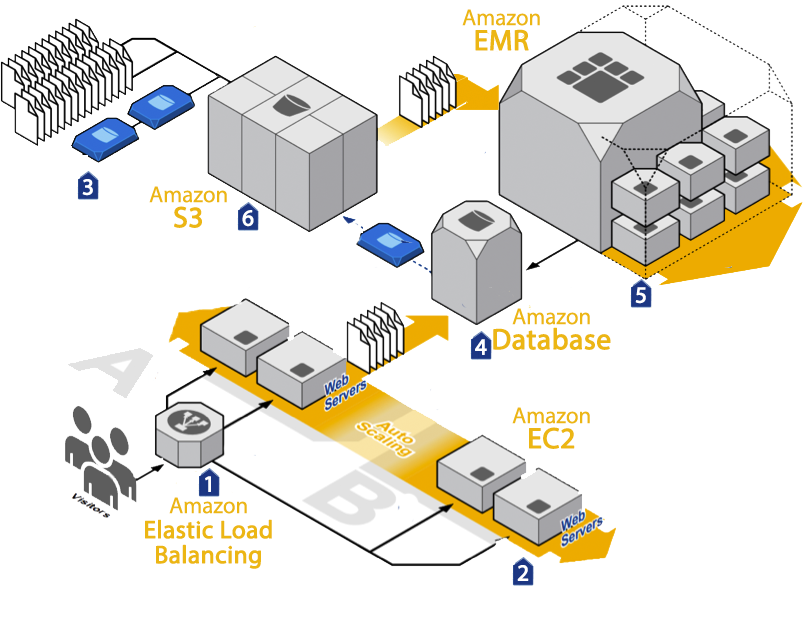
\includegraphics{arquitectura}
\caption{Arquitectura da Solução}
\label{fig:arquitectura}
\end{figure}


\section{Armazenamento dos dados dos Sensores}
O Cloud Weather processa grandes quantidades de dados recebidos em ficheiros de texto. Deste modo é possível processar dados oriundos de qualquer fonte, desde que devidamente formatados (as linhas em que o formato não é respeitado são ignoradas). Assume-se um formato standard da forma: <Cidade>, <Data>, <Hora>, <Temperatura>, <Humidade>, <Pluviosidade>.\\
Por simplificação, admitimos que os ficheiros de texto são gerados por uma aplicação exterior ao nosso serviço.
\section{Map-Reduce}
O algoritmo de Map-Reduce utilizado pelo Cloud Weather é simples e eficiente. O seu input é o ficheiro de texto, com o formato descrito na seção anterior, que se encontra guardado no Amazon Simples Storage Service (S3) no bucket: "ist.tagus.weather". O path para este ficheiro é definido pelo argumento do .jar que o Elastic Map-Reduce irá utilizar.\\
Cada instância de Mapper recebe uma porção dessas linhas do ficheiro de texto como input.  O conteúdo de cada linha é validado e processado. Caso o formato ou conteúdo da linha seja inválido, esta é ignorada. De modo a abstrair os dados recebidos pelo Reducer, o conteúdo de cada linha é convertido num objeto "WeatherWritable(temperatura, humidade, precipitação)" e é gerada uma chave constituída por "Cidade","Data". O output do mapper tem então como chave: "Cidade,Data" e um objecto WeatherWritable, por exemplo: <"Lisboa,2012-11-27",<4,95,10> >.\\
A escolha da chave não foi aleatória. Os output do Mapper são agregados por igualdade das chaves. Deste modo, todos os dados relativos a uma dada cidade num determinado dia são processados na mesma instância de Reducer. A hora de recolha da amostra foi desprezada porque não é relevante para a análise dos totais do dia.\\
Os dados (temperatura, humidade e pluviosidade) de cada cidade/dia são somados e contabilizados, no caso do Máximo e Mínimo, verificamos a cada iteração qual o valor maior e menor e registamos o resultado. Depois de finalizar todas as iterações, dividimos as somas da temperatura, huminadade e pluviosidade pelo número de pela contagem para obter as médias.\\
Podem ocorrer casos em que os dados enviados são somente parciais relativamente a 1 dia. Esse número de registos necessários por dia é definido com a variável  NSAMPLESEACHDAY - CloudReducer.java. Caso não tenhamos dados suficientes, o programa Java consulta o DynamoDB para procurar dados parciais desse dia que já tenham sido processados anteriormente. Caso existam, os dados são juntos à proporção que representam relativamente ao nº de amostras total. Admitimos que a soma das amostras parciais não excede o NSAMPLESEACHDAY, isto é, é aceite que os sensores enviem a informação em partes de não como um todo, mas caso isto aconteça, para termos dados estatísticos reais, precisamos que estes se mantenham sobre um nível mínimo, se não pode se dar o caso de apresentar estatísticas ao utilizador que não são reais, como por exemplo: Ter apenas os dados de uma manhã de um dia da pluviosidade e assumir que estes se mantêm para o resto do dia. Para evitar más interpretações, quando os dados não são suficientes, são armazenados numa base de dados em DynamoDB e disponibilizados ao público mediante da notificação de que podem não apresentar a verdade. \\
O resultado de cada Reducer é guardado num objeto "StatisticsWeatherWritable" que guarda as médias, máximos e mínimos associados a uma chave "Cidade,Data". Este resultado poderia ser escrito num ficheiro mas neste caso cada instância de Reducer escreve o seu resultado na base de dados em DynamoDB para que possa ser acedido pela aplicação web e consultado pelos utilizadores que se liguem a mesma.\\


\subsection{Análise de Desempenho}
Além de suportar falhas nas linhas de input e de suportar que os dados sejam enviados de forma parcial em diferentes períodos de tempo, temos um algoritmo que demonstra um desempenho dentro do esperado. Conseguimos processar 655 000 entradas em 29 minutos no Elastic Map Reduce com 4 máquinas small, o que dá uma média de 6550 linhas por minuto por máquina (admitindo 4 minutos para instanciação das máquinas). Tendo em conta que 24 amostras por dia em 18 capitais de distrito durante 1 ano resultam em 157 680 amostras para processar, o nosso algoritmo é suficiente para processar em tempo útil a quantidade de informação produzida por um país com 4x a dimensão de Portugal.\\
No entanto, a inicialização de máquinas para executar o MapReduce tem um custo temporal muito grande, instanciar os servidores e distribuir os dados por todos eles leva o seu tempo, criando uma latência de arranque que torna inviável utilizar este algoritmo para respostas tem tempo real.

\section{Sistemas de armazenamento na Cloud}
	Com aparecimento dos sistemas de computação distribuída em nuvem, o processamento de informação passou a ser feito em diferentes locais. De modo a tirar proveito do poder computacional distribuído geográficamente foi necessário alterar o paradigma de Storage existente. Foram criados novos tipos de bases de dados, designadas  bases de dados não relacionais(NoSQL), que permitem que a informação guardada seja distribuída e processada em diferentes locais, mantendo a mesma consistência dos dados. \\
	No entanto continuam a existem cenários em que é mais indicado usar-se os sistemas de Storage mais tradicionais como file system e bases de dados relacionais, sendo estes também oferecidos pelos provedores de computação na nuvem.\\
	Existem várias soluções NoSQL, como: graph bases, multimodel databases, object databases, grid database, xml database, multidimensional database, multivalue databace, event source, wide column store, document store e key value store, sendo as  3 últimas, as mais oferecidas no mercado de sistemas de storage na cloud.\\

\section{MongoDB VS DynamoDB}
	Durante o estudo de arquitetura para o desenvolvimento da aplicação Cloud Weather, analisamos várias soluções que nos pareceram ser indicadas para a solução final, sendo que por último a decisão foi feita entre o serviço de Document Store oferecido pela MongoDB da 10gen e o serviço de Key Value Store oferecido pela DynamoDB da Amazon.\\
	A MongoDB oferece um vasto leque de 'drivers', API que dão suporte ao desenvolvimento com várias linguagens de programação como C\#, Java, JavaScript, PHP, etc. Tem nativamente 'Auto-Sharding', que significa que consegue particionar a base de dados por vários locais sem comprometer a funcionalidade.\\
	No entanto trás uma enorme desvantagem, que é o facto de ser feita em JavaScript, isto significa que é single thread, tendo de recorrer a um serviço terceiro, como por exemplo o Apache Hadoop, sempre que quiser executar uma função MapReduce para processar uma grande quantidade de informação, isto claro, se quisermos ter os resultados em tempo prático.\\
	A DynamoDB é um serviço storage Key Value oferecida pela Amazon, o que oferece à priori a melhor integração com os serviços Cloud da Amazon, é escalável e tem um sistema nativo de tolerância a falhas e em comparação com a MongoDB, trás um sistema de MapReduce elástico que permite alocar de forma automática várias instancias de MapReduce consoante a dimensão dos dados a processar.\\
	Tendo tudo isto em conta e sabendo que iríamos usar unidades EC2 para o desenvolvimento do projeto, optamos por usar DynamoDB como serviço de Storage, pois este trás uma compatibilidade otimizada inerente às unidades da Amazon EC2.


%%------------------------------------------------------------------------------------------------------------------------------------------------


\section{Servidor Web}
Os utilizadores do Cloud Weather podem consultar os resultados Online. Para tal, instanciamos um servidor no Amazon Elastic Cloud Computing com uma Amazon Machine Image (AMI) genérica "Ubuntu Server 12.04.1 LTS". Esta imagem foi configurada com a instalação do Apache2, PHP5 e Java Developer Kit 6(JDK 6) para ser utilizada como WebServer.\\
O acesso Web é constituído por uma página PHP (weathersearch.php) e outra HTML + JS + PHP (index.php). A página principal (index.php) constitui a interface de utilizador. O utilizador indica os dados pretendidos sobre uma determinada cidade e dia e submete o seu pedido no formulário. Este formulário é lido pelo JavaScript e é submetido (POST) na página PHP weathersearch.php que por sua vez faz uma query ao DynamoDB pela HashKey Cidade e RangeKey Data. Como resultado é devolvida uma string formatada em JSON com os dados pretendidos. Esta string JSON é então analisada pelo Javascript e os dados são apresentados ao utilizador.\\
Foi utilizada uma arquitetura LAP (Linux + Apache + PHP) porque o seu desempenho e simplicidade são adequados às necessidades e ainda permitiu aprender a utilizar as ferramentas de desenvolvimento Amazon para PHP.\\
Poderíamos utilizar Internet Information Services (IIS) da Microsoft (numa arquitetura .NET) mas privilegiamos  a utilização de software livre. No caso do Google App Engine, utilizaríamos uma arquitetura Apache + Java Applets. \\
\\
\\
\section{Elastic Load Balancer e Route 53}
Quando se presta um serviço é quase sempre vital que este serviço esteja disponível o maior tempo possível. Se o serviço fosse fornecido por um único servidor e este falhasse ou ficasse sobrecarregado, o nosso serviço ficaria indisponível. Por isso replicamos o serviço por vários servidores aumentando a redundância. Mas não basta replicar, o utilizador não quer ter de descobrir qual o servidor disponível. Para que esta distribuição seja transparente ao utilizador, utilizamos um Load Balancer.\\
O Load Balancer pode ser implementado por hardware ou por software. Em ambos, o objetivo é distribuir os pedidos por um conjunto de recursos. Esta distribuição pode ser um simples Round Robin até a algoritmos mais complexos que tenham em conta a ocupação dos servidores, tempos de resposta ou outras métricas resultantes da monitorização dos recursos.\\
Um dos problemas dos Load Balancers é a manutenção de uma sessão. Supondo que queremos melhorar o serviço de Cloud Weather mantendo o histórico de pedidos do utilizador. É difícil manter os registos nos servidores em que estes são realizados porque o utilizador muito provavelmente não fará os pedidos sempre no mesmo servidor. Uma alternativa possível seria encaminharmos o utilizador sempre para o mesmo servidor (identificando o utilizador pelo seu username, IP ou um cookie no browser) mas se o servidor falhar, a sessão desaparece. Em alternativa podemos centralizar a informação numa base de dados.\\
A arquitetura de um load balancer pode ser bastante complexa, incluindo HealthChecking, Cache, Filtro de conteúdos, prioritização de trafego, Firewall, IPS, IDS, etc. No entanto é preciso ter bastante atenção para não tornar o próprio load balancer um bottleneck do sistema. Existem várias soluções de software de load balancing livre. No entanto, uma vez que estamos a usar unidades de computação EC2 da Amazon, optamos pelo Elastic Load Balancer. Não deixaria no entanto de ser bastante lúdico e interessante, compreender melhor este mecanismo de balanceamento de carga.
\\
\\
\begin{figure}[htb]
\centering
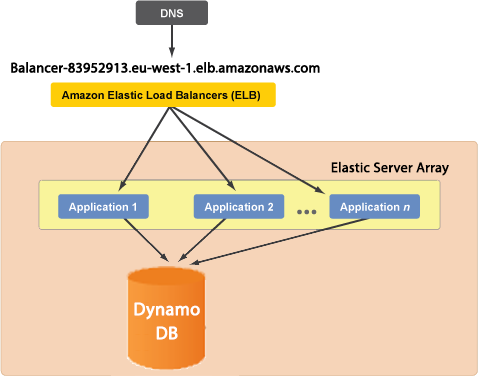
\includegraphics[scale=0.7]{webArch}
\caption{Arquitectura do Load Balancer}
\label{fig:webArch}
\end{figure}

\subsection{Configuração do Load Balancer}
Para configurar um Load Balancer através do Console Manager do AWS, começamos por configurar primeiro pelo menos 2 máquinas. O menu de configuração é bastante simples. \\
Foi-nos atribuído um DNS A Record:  balancer-604992545.eu-west-1.elb.amazonaws.com. Se quisermos registar um domínio mais simples, temos sempre de utilizar um CNAME para este DNS A Record (domínio) e não um IP porque não é garantido que seja sempre a mesma máquina a responder ao pedido.\\
Se quisermos ocultar o nome de DNS podemos utilizar o serviço Route 53. Este serviço não é mais do que um servidor DNS da Amazon. No entanto não o utilizamos porque ainda que a Amazon forneça um serviço "registrar" DNS, isto é, não possibilita o registo de domínios, apenas realiza a tradução DNS, ou seja teríamos de comprar o domínio em outro provedor. \\
Para testar a falha de um dos servidores, acedemos por SSH a um dos servidores e paramos o serviço de Apache. Como definimos como métrica a falha de 2 HTTP Request à página index.php de cada um dos servidores, o Load Balancer declara que um deles falhou. O domínio não fica indisponível porque o tráfego é direcionado para outro servidor. Além disso, o subtítulo da página é o nome do servidor por isso podemos ver que o nome do servidor que responde ao nosso pedido comuta.\\


\section{Auto-Scalling}
Na seção anterior confirmamos que no caso de uma das máquinas falhar, a carga é enviada para a outra máquina. Num cenário de Load Balancer estático com  2 máquinas a 50\% , se uma delas falhar a outra irá provavelmente falhar porque terá de suportar uma carga de 100\%. Por oposição, ter 3 máquinas a funcionar a 25\% temos um desperdício de 75\% da capacidade de computação.\\
Existem várias hipóteses para auto-scalling como por exemplo desligar o servidor atual quando este atingir a carga máxima e instanciar um novo com mais recursos mas deste modo o site fica em baixo durante alguns instantes que podem ser cruciais para o sucesso do negócio. No caso do AWS, iremos demonstrar que podemos monitorar e instanciar novos servidores em paralelo antes que os servidores atuais fiquem sobrecarregados. \\
Para resolver esta situação, utilizamos o Elastic Load Balancer da Amazon que permite auto-scalling do número de máquinas. O sistema é monitorizado em tempo real pelo 
Cloud Watch e em função das métricas que definimos, o serviço cria mais instâncias e distribui o tráfego por elas.\\
O auto-scalling deve ser muito bem planeado com base em estudos de padrões de utilização, em previsões de utilização devido a fatores econômicos (Natal, Black-Fridays, lançamento de novo produto) porque o problema não é a utilização continua e intensiva dos recursos mas sim os picos de tráfego. Como as máquinas têm um tempo de arranque, este boot-time é crucial para uma resposta atempada aos pedidos dos utilizadores. Se instanciarmos máquinas muito cedo, poderá ser um falso alerta, se instanciarmos tarde haverá utilizadores a ficar sem resposta.\\


\subsection{Configuração do Auto-Scalling}
Para que o número de instâncias do sistema seja auto escalável, é preciso configurar o Auto-Scalling. Todas as instâncias têm de escalar com a mesma Amazon Machine Image (AMI) com todo o sistema configurado à nossa medida e pronto a correr. \\
Temos 3 alternativas: podemos colocar os nossos ficheiros do WebSite num Elastic Block Storage (EBS) ou integrar os ficheiros numa Amazon Machine Image ou configurar a imagem para descarregar a versão mais recente a partir do S3. A 1ª solução permite-nos armazenar de 1GB até 1TB numa única drive virtual que pode ser atribuída a máquinas dentro da mesma Availability Zone e ainda oferece replicação dos dados. Na 2ª opção, os ficheiros ficam guardados como configuração da imagem. A 3ª permite que as novas instâncias corram sempre a versão mais recente mas exige configuração de uma política de updates nas máquinas existentes.\\
Optamos pela 2ª opção porque trata-se de um website estático que não requer atualizações. No caso da 3ª opção temos de ter em conta o atraso provocado no arranque e ainda que os downloads a partir do S3 são taxados.\\
\\
\\

Criámos uma AMI com id: ami-874f42f3.  Depois instalamos as "Auto Scalling tools" da Amazon e configuramos qual a instância que queremos que o auto-scale crie uma instância micro:

\lstset{language=Bash} 
\begin{lstlisting}
as-create-launch-config CloudWeatherLaunchConfFinal 
       --region eu-west-1
       --image-id ami-51434e25
       --instance-type t1.micro
\end{lstlisting}
De seguida definimos o grupo de máquinas que irá escalar segundo a configuração anterior. Definimos como propriedades que vamos aguardar 10 segundos entre lançar novas instâncias, aguardar 10 segundos para que as máquinas comecem a ser monitorizadas para que o Load Balancer "Balancer" (definido anteriormente) possa começar a encaminhar tráfego. Definimos que queremos no mínimo 2 instâncias e no máximo 10, nas availability-zones da Europa.\\


\lstset{language=Bash} 
\begin{lstlisting}
as-create-auto-scaling-group CloudWeatherAutoGroup 
	--launch-configuration CloudWeatherLaunchConf 
	--default-cooldown 10  
	--grace-period 10 
	--load-balancers  Balancer 
	--min-size 2 --max-size 10 
	--availability-zones eu-west-1a 
	--region eu-west-1
\end{lstlisting}


Definimos agora a nossa política para incrementar o nº de máquinas (incrementar 1 máquina e aguardar 30 segundos até que possamos fazer outro trigger):\\

\lstset{language=Bash} 
\begin{lstlisting}
as-put-scaling-policy 
	--auto-scaling-group CloudWeatherAutoGroup 
	--name scale-up --adjustment 1 
	--type ChangeInCapacity --cooldown 10
\end{lstlisting}
 E a nossa política de decrementar o nº de máquina uma uma unidade:

\lstset{language=Bash} 
\begin{lstlisting}
as-put-scaling-policy --auto-scaling-group CloudWeatherAutoGroup 
	--name scale-down "--adjustment=-1" 
	--type ChangeInCapacity --cooldown 30
\end{lstlisting}


Configuradas as ações, vamos agora automatizá-las. Para isso utilizamos o Cloud Watch da Amazon. O Cloud Watch monitoriza as instâncias de EC2 segundo os critérios que vamos definir e executará as ações definidas quando os valores de determinados parâmetros atingirem o valor definido no trigger.  Para isso utilizamos o comando mon-put-metric-alarm:\\

\lstset{language=Bash} 
\begin{lstlisting}
mon-put-metric-alarm 
	--alarm-name CloudWeather-scale-up-alarm
	--alarm-description "Scale up at 80% load"
	--metric-name CPUUtilization
	--namespace AWS/EC2 --region eu-west-1 
	--statistic Average  --period 60 --threshold 80 
	--comparison-operator GreaterThanThreshold 
	--evaluation-periods 3  --unit Percent
	--dimensions "AutoScalingGroupName= CloudWeatherAutoGroup"
	--alarm-actions arn:aws:autoscaling:eu-west-1:410572870616:scalingPolicy:
	8e010277-f338-477b-b304-10771fdc245d:
	autoScalingGroupName/CloudWeatherAutoGroup:policyName/scale-up
\end{lstlisting}

E o comando para reduzir o número de instâncias: 

\lstset{language=Bash} 
\begin{lstlisting}
mon-put-metric-alarm 
	--alarm-name CloudWeather-scale-down-alarm
	--alarm-description "Scale down at 20% load" 
	--metric-name CPUUtilization 
	--namespace AWS/EC2 
	--statistic Average  --period 60 --threshold 40 
	--comparison-operator LessThanThreshold --evaluation-periods 3  
	--unit Percent 
	--dimensions "AutoScalingGroupName= CloudWeatherAutoGroup" 
	--region eu-west-1 
	--alarm-actions arn:aws:autoscaling:eu-west-1:410572870616:scalingPolicy:
	45b5fe1f-03e4-486d-bc3d-429d7f759e89:
	autoScalingGroupName/CloudWeatherAutoGroup:policyName/scale-down
\end{lstlisting}


Estes 2 comandos descrevem um alarme que é lançado quando a métrica CPUUtilization está acima de 80\% ou abaixo de 40\% durante 60 segundos e nesse caso tem como ação a política de Auto-Scalling que definimos, incrementando ou decrementando, respectivamente, o número de instâncias.\\
 Para verificar a configuração: 
\lstset{language=Bash} 
\begin{lstlisting}
as-describe-auto-scaling-groups CloudWeatherGroup --headers
\end{lstlisting}

Uma das características mais interessantes de termos optado por um utilizar AMI's é de que podemos criar uma nova as-launch-config com uma nova AMI e fazer update ao scaling-group  para a nova AMI:\\
\lstset{language=Bash} 
\begin{lstlisting}
/as-update-auto-scaling-group CloudWeatherAutoGroup 
	 --launch-configuration CloudWeatherLaunchConf3
\end{lstlisting}
O mais relevante é que para comutarmos para a nova imagem, podemos desligar os servidores para um número inferior ao mínimo do Auto Scaller que este irá instanciar de imediato novos servidores com a imagem mais recente permitindo uma atualização simples e sem interrupção de serviço.


\subsection{Load Script}
De modo a testar o Auto Scalling e o Load Balancer utilizamos 2 ferramentas com métodos distintos mas com o mesmo objetivo: sobrecarregar o servidor e fazer com que o Cloud Watch lance o alarme que faz o auto-scaller lançar novas instâncias.\\
Uma das ferramentas foi criada pelo nosso grupo. Trata-se de um programa java que cria várias threads para executar POST's (pedidos HTTP) ao servidor.\\
Em alternativa utilizamos o Siege. O Siege faz um número de GET's assíncronos em paralelo para testar o Apache levando à sobrecarga do servidor.O comando siege apresentado define 25 clientes durante 10 minutos a fazer get do URL apresentado.\\
\lstset{language=Bash} 
\begin{lstlisting}
siege -c25 -t10M  http://balancer-604992545.eu-west-1.elb.amazonaws.com
\end{lstlisting}
No entanto os resultados apresentados não eram satisfatórios, devolver o resultado de uma query ao dynamoDB ou devolver uma página quase 100\% estática, não exige muita performance de CPU e exige uma grande quantidade de mensagens e de tráfego de rede. Como tal, criamos o script: "factor.php" que realiza a factorização de um número grande e ainda faz 100 digests MD5 a uma string aleatória de 1000 caracteres. Deste modo o sistema entra rapidamente em sobrecarga.\\
Isto permitiu-nos concluir que a vulnerabilidade a ataques mais do que do número de pedidos, depende do processamento exigido ao servidor por esse número de pedidos.\\
Um outro aspecto ainda a ter em conta é o checker do load balancer. Este "keep-alive" query deve ser feito a uma página que não exija processamento porque caso contrário irá manter o processador ocupado a consumir recursos desnecessariamente. No nosso caso, o keep-alive do balancer à página com factorização de 30 em 30 segundos manteve a média de ocupação do servidor em 40\% sem nenhum outro cliente.



\section{Análise de Performance}
O auto-scalling permite-nos utilizar um grande número de métricas para monitorizar o sistema e para escalar o número de instâncias. No entanto nesta análise de performance vamos focar-nos apenas numa métrica: Utilização de CPU; porque estamos interessados em testar a resposta do sistema em caso de sobrecarga e como devemos dimensionar os alarmes para que o sistema não deixe de responder aos utilizadores mas também não desperdice recursos. \\
Vamos prever então 3 tipos de tráfego:
   \begin{itemize}
\item Rajadas pontuais - Abertura das inscrições para o IST, lançamento de um novo telemóvel, eventos com inicio definido no tempo que amplamente divulgados, em que ser o 1º a realizar trás vantagens ao utilizador.
\item Rajadas incrementais durante um intervalo - Notícias que são divulgadas rapidamente e que trazem um número cada vez maior de utilizadores num curto espaço de tempo.
\item Utilização variável - Site normal com períodos de pico e de baixa utilização\end{itemize}

A tabela \href{table:Parametros} resume os principais parametros que podemos utilizar para configurar o auto-scaling.

\begin{table}[ht]
\centering
\begin{tabular}{| c | p{10cm} |}
    \hline
    {\bf Métrica } & {\bf Descrição }  \\ \hline\hline
    {\bf Auto-Scaling-Group} &  \\ \hline
	 default-cooldown & Tempo entre escalamentos \\ \hline
	 grace-period &  Período em que o load-balancer ignora se a instância não responder\\ \hline

	min-size &  Dimensão minima do Grupo \\ \hline
	max-size &  Dimensão máxima do Grupo \\ \hline\hline
	
	{\bf Scaling-Policy } &  \\ \hline
	 adjustment &  Quantas instancias? \\ \hline
	 cooldown &  Intervalo entre aplicações desta politica \\ \hline\hline
	{\bf Metric Alarm } &  \\ \hline
	 comparison-operator  &  GreaterThanOrEqualToThreshold,  GreaterThanThreshold, 
       LessThanThreshold and LessThanOrEqualToThreshold \\ \hline
	threshold &  threshold da metrica que iremos comparar\\ \hline
	 statistic &  Estatistica da métrica: SampleCount, Average, Sum, Minimum, Maximum. \\ \hline
	evaluation-periods  &  Número de vezes que a métrica é comparada até lançar o alarme \\ \hline
period  &   Período de verificação da métrica\\ \hline
    \hline
  \end{tabular}
\caption{Parametros para ajustar o auto-scaling}
\label{table:Parametros} % usado para referir esta tabela no texto
\end{table}

Estes parâmetros serão configurados nas próximas subsecções com vista à resposta aos vários casos de estudo. Para acelerar o processo de testes, foi desenvolvido o script de configuração (Apêndice A).


\subsection{Rajadas momentâneas}
No caso de rajadas momentâneas, o fator mais importante é termos uma resposta rápida que se ajuste depressa às alterações no número de utilizadores por isso vamos otimizar a configuração.\\
Visto que prevemos uma rajada, vamos prevenirmos colocando aumentando o número mínimo e máximo de máquinas no grupo. Além disso vamos escalar com mais máquinas de cada vez (adjustment) e com menor cooldown. Queremos reagir o mais cedo possível por isso o threshold superior deve ser baixo e avaliado.\\
Realizamos um teste com um grupo de 4 a 15 máquinas que aguarda apenas 10 segundos entre lançar mais 3 instâncias. Isto exige um acompanhamento mais rigoroso do Cloud Watch.
\begin{table}[ht]
\centering
\begin{tabular}{| c | p{3cm} | p{3cm} |}
    \hline
    {\bf Métrica} & \multicolumn{2}{|l|}{ {\bf Valor}} \\ \hline
    \multicolumn{3}{|l|}{ {\bf Auto-Scaling-Group}} \\ \hline
	 default-cooldown & \multicolumn{2}{|c|}{ 10 sec }\\ \hline
	 grace-period &  \multicolumn{2}{|c|}{ 60 sec } \\ \hline

	min-size &   \multicolumn{2}{|c|}{ 4  } \\ \hline
	max-size &   \multicolumn{2}{|c|}{ 15 }\\ \hline\hline
		
	{\bf Scaling-Policy } & {\bf Upgrade } & {\bf Downgrade }  \\ \hline\hline
	
	 adjustment &  +3       & -3     \\ \hline
	 cooldown &  10sec & 10sec  \\ \hline\hline
	
	
	\multicolumn{3}{|l|}{ {\bf Metric Alarm}} \\ \hline
	 comparison-operator  &  GreaterThan & LessThan \\ \hline
	 threshold &  50  & 20 \\ \hline
	 statistic &  Maximum & Maximum \\ \hline
	 evaluation-periods  &  1 & 1 \\ \hline

	period  &   60 sec & 60 sec \\ \hline		
  \end{tabular}
\caption{Parametros para auto-scaling de rajadas}
\label{table:ParametrosRajadas} % usado para referir esta tabela no texto
\end{table}



\begin{table}[ht]
\centering
\begin{tabular}{| c | c |}
    \hline
    {\bf Métrica} &  {\bf Valor} \\ \hline
	Siege  Threads 		&  100  \\ \hline
	Siege  Duration 	&  10 m \\ \hline\hline
	Transactions 		&  22211 \\ \hline
	Availability 		&  95.67 \% \\ \hline
	Response time 		&  2.19 secs  \\ \hline
	Transaction rate 	&  24.68 trans/sec \\ \hline
	Failed transactions &  1005 \\ \hline
	Longest transaction &  29.97 \\ \hline
	Shortest transaction &  0.10 \\ \hline
  \end{tabular}
\caption{Resultados do Teste}
\end{table}


Na 1ª execução, apenas com máquinas micro, o sistema demorou 6 minutos a instanciar 11 máquinas até atingir o máximo de 15. Mesmo assim, as 16 máquinas não conseguiram responder às 10 clientes que neste intervalo realizaram, 22211 pedidos dos quais 5\% falharam. Em certos instantes o site é considerado indisponível. 
Vamos testar os limites deste sistema de 16 máquinas colocando 2 instancias Amazon com 300 threads cada uma. 

\begin{table}[ht]
\centering
\begin{tabular}{| c | c |}
    \hline
    {\bf Métrica} &  {\bf Valor} \\ \hline
	Siege  Threads 		&  2x300  \\ \hline
	Siege  Duration 	&  10 m \\ \hline\hline
	Transactions 		& 2664  \\ \hline
	Availability 		&  0.45 \% \\ \hline
	Response time 		&  606.89 secs  \\ \hline
	Transaction rate 	&  0.12 trans/sec \\ \hline
	Failed transactions &  2646 \\ \hline
	Longest transaction &  27.76 \\ \hline
	Shortest transaction &  18.95 \\ \hline
  \end{tabular}
\caption{Resultados do Teste}
\end{table}
O serviço ficou claramente indisponível mesmo escalando. O gráfico \href{fig:teste2CPU} demonstra claramente que durante todo o intervalo do teste, o sistema teve ocupação de 100%.\\

\begin{figure}[htb]
\centering
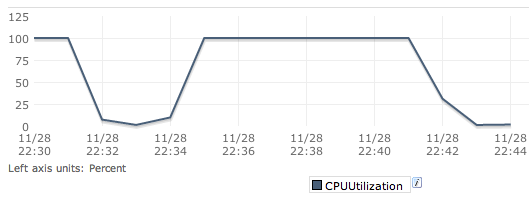
\includegraphics[scale=0.8]{teste1}
\caption{Gráfico de utilização do CPU durante o teste}
\label{fig:teste1CPU}
\end{figure}

O facto de termos instâncias micro limita a capacidade do sistema.\\
Repetindo o mesmo teste mas instanciando máquinas small e com mais tempo de execução.
\begin{table}[ht]
\centering
\begin{tabular}{| c | c |}
    \hline
    {\bf Métrica} &  {\bf Valor} \\ \hline
	Siege  Threads 		&  2x300  \\ \hline
	Siege  Duration 	&  15 m \\ \hline\hline
	Transactions 		& 2969  \\ \hline
	Availability 		&  13.48 \%  \\ \hline
	Response time 		&  23ms secs  \\ \hline
	Transaction rate 	&  2.24 trans/sec \\ \hline
	Failed transactions &  2641 \\ \hline
	Longest transaction &  29.97 \\ \hline
	Shortest transaction &  0.40 \\ \hline
  \end{tabular}
\caption{Resultados do Teste com instâncias 15 small}
\end{table}

Os resultados são mais satisfatórios, especialmente se tivermos em conta que ao fim de 10 minutos o número de servidores é suficientemente grande para conseguir começar a diminuir a intensidade de CPU.\\
\begin{figure}[htb]
\centering
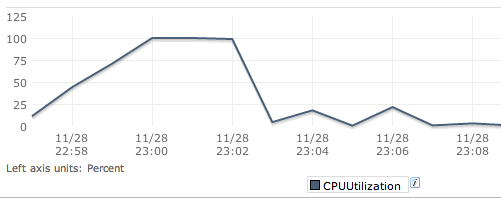
\includegraphics[scale=0.8]{teste2}
\caption{Gráfico de utilização do CPU durante o teste}
\label{fig:teste2}
\end{figure}

Esperando que tenhamos os 15 servidores disponíveis para correr os testes, verificamos pela tabela \href{tabela:teste3} que estes conseguem lidar perfeitamente com a carga imposta. 
\begin{table}[ht]
\centering
\begin{tabular}{| c | c | c |}
\hline
 {\bf Métrica} &  {\bf Valor Server 1}  &  {\bf Valor Server 2} \\  \hline
	Siege  Threads 		& 300   & 300\\ \hline
	Siege  Duration 	&  15 m &  15m\\ \hline\hline
	Transactions 		& 3774  & 3787\\ \hline
	Availability 		&  100.00 \% & 99.97 \%  \\ \hline
	Response time 		&  10.31 & 10.32  \\ \hline
	Transaction rate 	&  26.52 trans/sec & 26.57 trans/sec \\ \hline
	Failed transactions &  0 & 1 \\ \hline
	Longest transaction &  27.15 & 27.23 \\ \hline
	Shortest transaction &  2.81 & 3.01 \\ \hline
  \end{tabular}
\caption{Resultados do Teste com instâncias 15 small}
\label{tabela:teste3}
\end{table}
Um aspecto bastante interessante desta tabela (e homologo dos dados recolhidos nas experiências anteriores)é o facto de termos 2 clientes a tentar sobrecarregar os servidores mas o load balancer consegue distribuir os recursos equitativamente por ambos os clientes. Esta característica é boa ou má consoante a aplicação: no caso de termos um web site para consulta de uma noticia ou um conteúdo pontual é importante que todos os clientes sejam atendidos para que possam ver algum conteúdo enquanto o sistema escala no entanto em aplicações como por exemplo sessões numa loja virtual ou inscrições num curso, é preferível dar prioridade a quem já está registado para que complete a tarefa o mais rápido possível deixando o sistema livre para os seguintes. Existem várias opções para autenticar e identificar os utilizadores. No entanto este aspecto não é configurável na Amazon e está fora do âmbito deste documento. \\
Em ambos os casos, o sistema demora cerca de 10 minutos a remover todas as instâncias de servidores requisitados. Este tempo é aceitável e previne novas sobrecargas do sistema.\\
No entanto o minuto e meio que o sistema leva a começar a instanciar novos servidores é importante consoante o serviço que estamos a disponibílizar. Uma solução para evitar este problema é configurar um cluster de reserva que só entra em utilização quando a carga é elevada, suportando o intervalo necessário para instanciar os novos servidores. 

\subsection{Rajadas incrementais durante um curto intervalo}
Através dos resultados da experiência anterior podemos inferir as características necessárias para esta situação. Como demonstramos, desde que o sistema tenha tempo para escalar, conseguimos lidar com qualquer rajada de pedidos. Neste caso, o sistema reage mais facilmente porque podemos colocar um alerta mais baixo e começar a escalar mais cedo.

\subsection{Utilização variável}
No caso de uma utilização variável do site mas sem picos, o auto-scalling da Amazon é ideal. Durante os períodos de menor utilização, como por exemplo as madrugadas, reduz o número de instâncias. Durante a utilização normal mantém um número aproximadamente constante de instâncias. \\
Neste caso, é preferível ter uma instância com maiores recursos que absorva as oscilações de tráfego ao longo do dia para evitar a criação e remoção constante de instâncias menores que são pagas hora a hora.\\





%!TEX encoding = UTF-8 Unicode
% Chapter 3

\chapter{Conclusões} 
\label{Chapter4} 

\lhead{Chapter 4. \emph{Conclusões} }
A utilização dos Amazon Web Services permitiu criar uma arquitetura escalável com capacidade de processamento para grandes quantidades de dados e disponibilizar um serviço web escalável, garantindo o máximo de disponibilidade para o cliente. \\
Um dos desafios da realização do projeto com o Amazon Web Services foi a falta de documentação objetiva. A documentação da Amazon é na maior parte das vezes bastante redundante, com pouco detalho técnico e com imenso conteúdo de marketing, sendo difícil responder à questão pela qual procuramos. Isto criou um esforço extra para elaborar soluções como por exemplo um servidor web escalável, que é algo comum nas aplicações web hoje em dia. No entanto uma vez passado o período de aprendizagem da plataforma, a interface, a API Java e as Command Tools são bastante poderosas e simples.\\
\\
O auto scalling é baseado na recolha periódica do estado do sistema. Isto é muito ineficiênciente a nível de escalonamento porque é necessário aguardar que sejam recolhidos os dados para tomar a decisão de escalar o sistema ou não. Isto cria um maior atraso na capacidade de resposta. Este sistema de analise por 'polling' tem um limite mínimo de recolha de informação de 1 em 1 minuto. Se a este intervalo somarmos o tempo necessário para o arranque de uma máquina até que esta fique operacional, o intervalo mínimo para responder à alteração é considerável e mais do que suficiente para levar a um utilizador a desistir de utilizar o serviço.\\
\\
A utilização da Amazon Web Services  (IaaS) faz com que a  portabilidade do nossos sistema não fique muito limitada. Se quiséssemos passar o sistema para outro provedor ou para o nosso próprio datacenter teríamos de replicar os serviços de load balancer e auto-scaling oferecidos pela Amazon. Uma solução para este problema seria ter adoptado uma solução híbrida (local+cloud), como é o caso do Eucalyptus, em que quando as máquinas do cluster local não são suficientes, escala para a Cloud. \\
\\
Caso este projeto tivesse sido desenvolvido com o âmbito comercial, deveria ser feito um estudo intenso a nível financeiro, pois ao adotarmos a Amazon Web Services, ficamos impossibilitados de migrar o nosso serviço para uma solução de outros provedores de larga escala como o Microsoft Azure ou o Google App Engine. Uma vez que estes não dispõe dos mesmos serviços como por exemplo o DynamoDB, teriamos de utilizar os serviços disponíveis pelo outro provedor.\\
A solução final é adequada aos requisitos apresentados, é escalável, eficiente e simples de atualizar.
 
%\input{./Chapters/Chapter5} 
%\input{./Chapters/Chapter6} 
%\input{./Chapters/Chapter7} 

%----------------------------------------------------------------------------------------
%	THESIS CONTENT - APPENDICES
%----------------------------------------------------------------------------------------

\addtocontents{toc}{\vspace{1em}} % Add a gap in the Contents, for aesthetics

\appendix % Cue to tell LaTeX that the following 'chapters' are Appendices

%!TEX encoding = UTF-8 Unicode
% Appendix A

\chapter{Script de Configuração do Auto-Scaling} 

\label{anexoA} 

\lhead{Anexo A. \emph{Script de Configuração do Auto-Scaling}} 

\lstset{language=bash,breaklines=true} 
\begin{lstlisting}
#!/bin/bash

LAUNCH_CONFIGURATION=CloudWeatherLaunchConfFinal
AUTOSCALING_GROUP=CloudWeatherAutoGroup

#Tempo entre escalamentos
ASG_COOLDOWN=10
#Periodo em que o load-balancer ignora se a instancia nao responder
ASG_GRACE_PERIOD=60
#Dimensao minima do Grupo
ASG_MIN=4
#Dimensao maxima do Grupo
ASG_MAX=15
#Quantas instancias para incrementar?
ADJUSTMENT_UP=3
#Intervalo entre incrementos
SCALING_POL_COOL_UP=10

#Quantas instancias para decrementos?
ADJUSTMENT_DOWN=-3
#Intervalo entre decrementos
SCALING_POL_COOL_DOWN=10

#Periodo de verificacao
ALARM_PERIOD_UP=60
#Threashold
ALARM_THRESHOLD_UP=50
#Num de avaliacoes necessarias
ALARM_NUM_EVALUATION_UP=1
#Tipo de estatistica SampleCount, Average, Sum, Minimum, Maximum.
ALARM_STATISTIC_UP=Maximum

#Periodo de verificacao
ALARM_PERIOD_DOWN=60
#Threashold
ALARM_THRESHOLD_DOWN=20
#Num de avaliacoes necessarias
ALARM_NUM_EVALUATION_DOWN=1
#Tipo de estatistica  SampleCount, Average, Sum, Minimum, Maximum.
ALARM_STATISTIC_DOWN=Maximum

#Delete old data

as-delete-policy scale-up --auto-scaling-group $AUTOSCALING_GROUP
as-delete-policy scale-down --auto-scaling-group $AUTOSCALING_GROUP
as-delete-auto-scaling-group $AUTOSCALING_GROUP --force-delete
as-delete-launch-config $LAUNCH_CONFIGURATION

sleep 15
#Create new
as-create-launch-config $LAUNCH_CONFIGURATION --region eu-west-1 --image-id ami-51434e25 --instance-type t1.micro
as-create-auto-scaling-group $AUTOSCALING_GROUP 	--launch-configuration $LAUNCH_CONFIGURATION --default-cooldown $ASG_COOLDOWN --grace-period $ASG_GRACE_PERIOD --load-balancers  Balancer --min-size $ASG_MIN --max-size $ASG_MAX --availability-zones eu-west-1a --region eu-west-1
sleep 5 
ACTION_UP=$(as-put-scaling-policy --auto-scaling-group $AUTOSCALING_GROUP --name scale-up --adjustment $ADJUSTMENT_UP --type ChangeInCapacity --cooldown $SCALING_POL_COOL_UP)
ACTION_DOWN=$(as-put-scaling-policy --auto-scaling-group $AUTOSCALING_GROUP --name scale-down --adjustment=$ADJUSTMENT_DOWN --type ChangeInCapacity --cooldown $SCALING_POL_COOL_DOWN)
sleep 5


mon-put-metric-alarm --alarm-name CloudWeather-scale-up-alarm --alarm-description "Scale up at $ALARM_THRESHOLD_UP % load" --metric-name CPUUtilization --namespace AWS/EC2 --region eu-west-1  --statistic $ALARM_STATISTIC_UP  --period $ALARM_PERIOD_UP --threshold $ALARM_THRESHOLD_UP --comparison-operator GreaterThanThreshold --evaluation-periods $ALARM_NUM_EVALUATION_UP  --unit Percent --dimensions "AutoScalingGroupName= $AUTOSCALING_GROUP" --alarm-actions $ACTION_UP
mon-put-metric-alarm --alarm-name CloudWeather-scale-down-alarm --alarm-description "Scale down at $ALARM_THRESHOLD_DOWN % load"  --metric-name CPUUtilization  --namespace AWS/EC2  --statistic Average  --period $ALARM_PERIOD_DOWN --threshold $ALARM_THRESHOLD_DOWN  --comparison-operator LessThanThreshold --evaluation-periods $ALARM_NUM_EVALUATION_DOWN   --unit Percent --dimensions "AutoScalingGroupName= AUTOSCALING_GROUP" --region eu-west-1 --alarm-actions $ACTION_DOWN
\end{lstlisting}
%\input{./Appendices/AppendixB}
%\input{./Appendices/AppendixC}

\addtocontents{toc}{\vspace{1em}} % Add a gap in the Contents, for aesthetics

\backmatter

%----------------------------------------------------------------------------------------
%	BIBLIOGRAPHY
%----------------------------------------------------------------------------------------

%\label{Bibliography}

%\lhead{\emph{Bibliography}} % Change the page header to say %"Bibliography"

%\bibliographystyle{unsrtnat} % Use the "unsrtnat" BibTeX style for formatting the Bibliography

%\bibliography{Bibliography} % The references (bibliography) information are stored in the file named "Bibliography.bib"

\end{document}  